
\begin{abstract}
Algorithmic processing of web content mostly works on textual contents, neglecting visual information.
Annotation tools mostly share this deficit as well.

We specify requirements for an architecture to overcome both problems and propose an implementation, the \KrdWrd~system.
It uses the Gecko rendering engine both for annotation and for feature extraction, providing unified data access in any processing step.
Stable data storage and collaboration control scripts for group annotations of massive corpora are provided via a web interface coupled with a HTTP proxy.
A modular interface allows plugging in feature extractors for linguistic and visual data.

The implementation is suitable for many tasks in the web as corpus domain and beyond.
\end{abstract}

\section{Introduction}
Working with algorithms that rely on user-annotated web content suffers from two major deficits:

For annotators, the presentation of web sites in the context of annotation tools usually does not match their everyday web experience.
The lack or degeneration of non-textual context may negatively affect the annotators' performance
and the learning requirements of special annotation tools may make it harder to find and motivate annotators in the first place.

Feature extraction performed on annotated web pages on the other hand leaves much of the information encoded in the page unused,
mainly those concerned with rendering.

In this paper, we present the design (\ref{design}) and implementation (\ref{impl}) of the {\KrdWrd} architecture that addresses these two issues.
Section \ref{casestudy} demonstrates a show-case in the context of the CleanEval challenge and Section \ref{conc} concludes with an outlook on the possible applications and implementation improvements.


\section{Design\label{design}}
\subsection{Design Goals}

We want to provide an architecture for Web data processing that is based on unified treatment of data on annotation and processing side
and that allows the back-end machinery to access all information contained in a Web page, including how it is presented to a Web surfer.

\subsection{Requirements}

\begin{description}

\item[Flexibility]
The system should be open enough to allow customization of every part, but also specifically provide stable interfaces for more common tasks to allow for modularization.

\item[Stability]
We need a stable HTTP data source that is independent of the original Website, including any dependencies such as images, style-sheets or scripts.

\item[Automaticity]
Back-end processing should run without requiring any kind of human interaction.

\item[Replicability]
Computations carried out on Web pages' representation must be replicable across systems, including any user-side processing.

\item[Quantity]
Corpus size should not influence the performance of the system and total processing time should grow linearly with the corpus.

\item[Usability]
Usability of the annotators side is of paramount importance, so we should stay as close as possible to the everyday Web experience.
We also need to provide tools for learning how to use the annotation tool and how to annotate Web pages.

\end{description}

\subsection{Core Architecture}

To address these requirements, we developed an abstract architecture, a simplified version of which is depicted in figure \ref{f:arch}.
We will outline the rationale for the basic design decisions below.


For rendering a Web page, an object tree is constructed from its HTML source code.
This tree can be traversed and its nodes inspected, modified, deleted and created through an API specified by the World Wide Web Consortium's (W3C) DOM Standard \cite{dom}.
It's most popular use case is client-side dynamic manipulation of Web pages, for visual effects and interactivity.
This is most commonly done by accessing the DOM through a JavaScript interpreter.
Essentially, a page's DOM tree allows access to all the information we set out to work on: structure, textual content and visual rendering data.
We therefore make it the sole interface between application and data.

While all browsers try to implement some part of the DOM standard (currently, version 3 is only partially implemented in most popular browsers), they vary greatly in their level of compliance as well as their ability to cope with non-standard compliant content.
This leads to structural and visual differences between different browsers rendering the same Web page.

Therefore, to guarantee \textit{replicability}, we require the same DOM engine to be used through the system.


To reach a maximal level of \textit{automaticity} and not to limit the \textit{quantity} of the data, it is important that data analysis can take place in a parallel fashion and does not require any kind of graphical interface, so it can e.g. be executed on server farms.
On the other hand we also need to be able to present pages within a browser to allow for user annotation.

Consequently, the same DOM engine needs to power a browser as well as a headless back-end application, with \textit{usability} being an important factor in the choice of a particular browser.


The annotation process, especially the order of presentation of pages, is controlled by a central Web server.
Thereby any number of concurrent annotators can be coordinated and submissions distributed equally across corpora.
All data, un-classified and user-submitted, is stored in a database attached to the Web server.
This setup allows the architecture to scale \textit{automatically} with user numbers under any usage pattern and submission \textit{quantity}.


\textit{Stability} of data sources is a major problem when dealing with Web data.
As we work on Web pages and the elements contained in them, simple HTML dumping is not an option.
Instead, we use a HTTP proxy to cache Web data used in our own storage.
By setting the server to grab content only upon first request and providing a option to turn off download of new data, we can create a closed system that does not change anymore once populated.


\begin{figure}
\jss{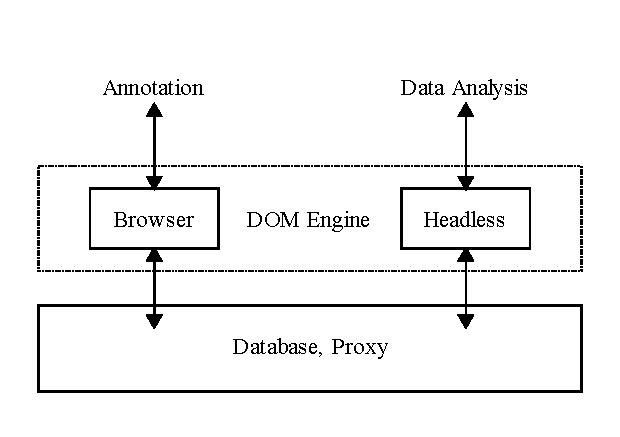
\includegraphics[width=0.4\textwidth]{arch}}
	{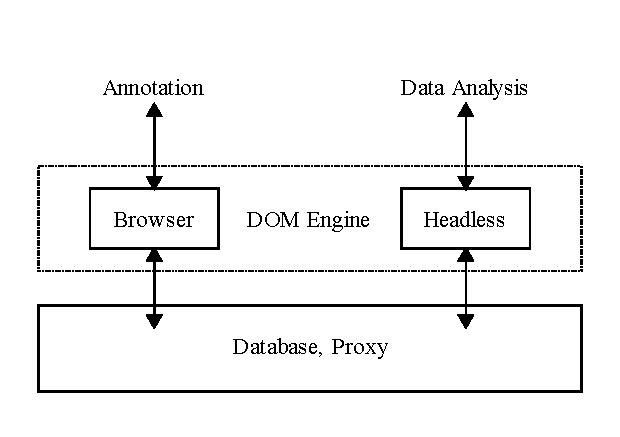
\includegraphics[width=0.8\textwidth]{arch}}
\caption{\label{f:arch}Basic {\KrdWrd} architecture: both users annotating corpus pages through their Web browser
and back-end applications working on the data run the same DOM engine.
	The central server delivers and stores annotation data and coordinates user submissions.}
\end{figure}




\section{Implementation\label{impl}}

We maintain the implementation in a source code repository at \url{http://krdwrd.org}.
The documentation includes pointers to required external software.

This section will first describe the DOM engine and its use by browser and backend application (\ref{dom}).
\ref{server} details the implementation of central storage and control and \ref{extract} lists possible feature extractors for the backend.


\subsection{DOM Engine}

KHTML/WebKit (KDE, Apple), JavaScriptCore or V8 (Google);
The Gecko engine (Mozilla Corporation) and it's JavaScript implementation Spidermonkey;
We briefly checked on Presto (Opera) and Trident (Microsoft), but discarded them due to their proprietary nature.

\subsubsection{Firefox AddOn}

To avoid interference with other AddOns and existing configuration, we suggest creating a new browser profile for use with the AddOn.
For easy use, Firefox' proxy configuration is automatically pointed to a preconfigured host and the user is directed to a special landing page upon successful installation.
visual tagging, results

\begin{figure}
\jss{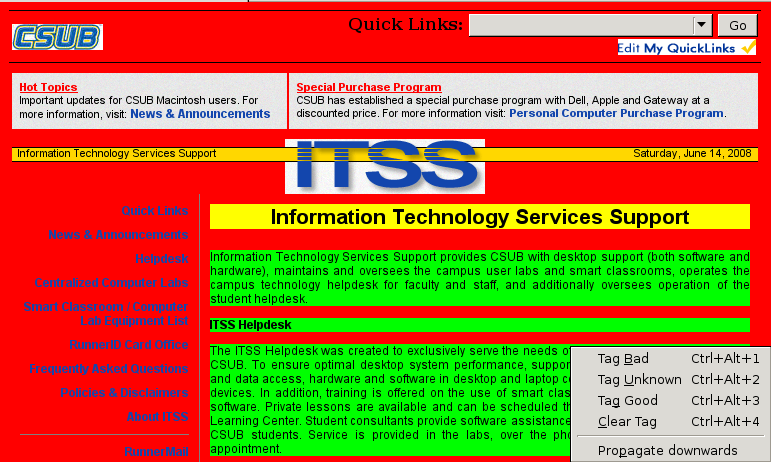
\includegraphics[width=0.5\textwidth]{tut0}}
	{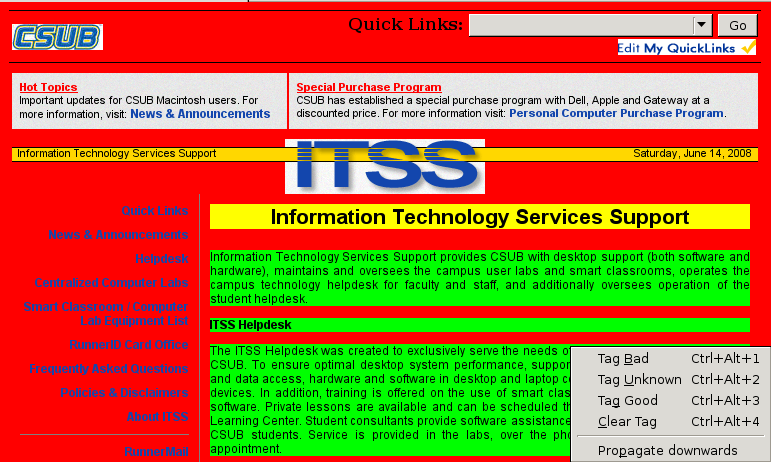
\includegraphics[width=\textwidth]{tut0}}
\caption{\label{f:tut0}Web pages can be annotated with the KrdWrd Firefox AddOn by hovering over the text by mouse and setting class labels by keyboard shortcut or pop-up menu}
\end{figure}


\subsubsection{XUL Application}

The XUL application (or \textit{app} for short) 
Dumper, Grabber, Crawler

% ens said: if you like:
% \cite{NajorkHeydon2001,ShkapenyukSuel2002}

\subsection{Storage and Control}

database and web server. 

\subsubsection{Web Server}

small Python CGI scripts;
provides per-corpora submission list,
controls serving of random corpus pages;
tutorial mode: visual diff after submit;
ssl connections only;

\begin{figure}
\jss{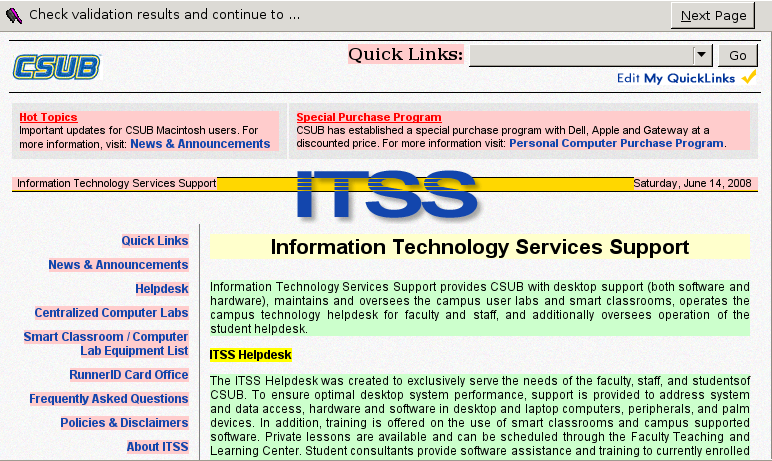
\includegraphics[width=0.5\textwidth]{tut1}}
	{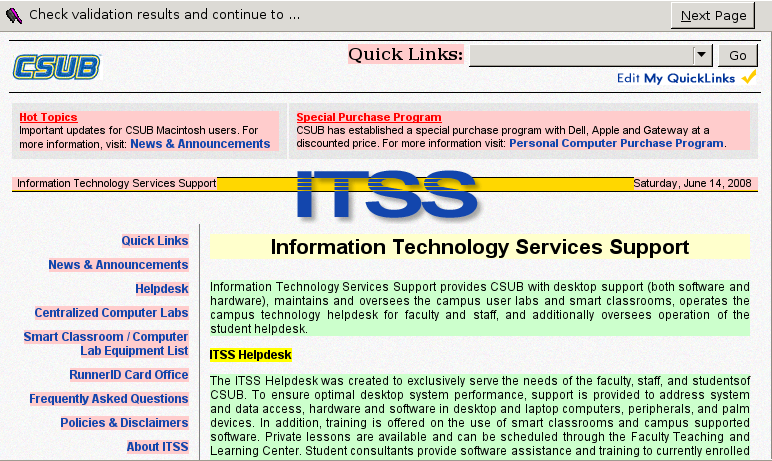
\includegraphics[width=\textwidth]{tut1}}
\caption{\label{f:tut1}During the tutorial, a Visual Diff between the user's submission and the sample data is presented right after submission.
	Here, the annotation from \ref{f:tut0} was wrong in tagging the sub-heading ``ITSS Helpdesk'': the correct annotation (\textit{yellow}) is highlighted in the feedback.}
\end{figure}

\subsubsection{Database}

Raw HTML in sqlite3;
user submissions are anonymized, but trackable by id;

\subsubsection{Proxy}

\begin{figure}
\jss{
\includegraphics[width=0.5\textwidth]{add}}
	{
\includegraphics[width=\textwidth]{add}}
\caption{IFrames with dynamic URLs which usually come from advertisements are blocked as a nice side-effect of the Proxy setup}
\end{figure}

\subsection{Feature Extractors}

app produces input files for pipelines, dumped in the filesystem, per-page with one line per dom text node;
integrated dom feature extraction;
integrated screen grab;

\subsubsection{Text}

Dumped raw text, leading and trailing whitespace removed, UTF-8.

\subsubsection{Meta Visual}

Use data from living DOM Tree in XUL App.

\subsubsection{Visual}

Screenshot and use JAMF as seen in \cite{Steger08}
\footnote{This Extractor requires at least XULRunner Version 1.9.2 (corresponding to Firefox Version 3.5) which is still in beta at the time of this writing}

\subsection{Machine Learner}

Generic input vectors and classes from extractors

\subsection{\label{sec:limitations}Highlights and Limitations}

html, utf, js, iframes


\section{Case Study\label{casestudy}}

We tested the implementation on a typical web-as-corpus task, including corpus creation, user annotation, feature extraction, traning a classifier and producing annotated test results.
The underlying data and programs are bundled with the {\KrdWrd} distribution as usage example.

\subsection{Data Acquisition\label{datagather}}

We acquired a new corpus named \textit{Canola} by using the BootCaT \cite{bootcat} tool to produce an URL list from the seed terms in table \ref{t:seed} using the Yahoo search engine. 

\begin{table}
\label{t:seed}
\centering
\jss{
\caption{BootCaT seed terms for \textit{Canola} corpus}\bigskip}{
\captionabove{BootCaT seed terms for \textit{Canola} corpus}\sffamily}
\begin{tabular}[h]{ccc}
        history
&        coffee 
&        salt \\
        spices 
&        trade road
&        toll \\
        metal
&        silk 
&        patrician \\
        pirate 
&        goods
&        merchant 
\end{tabular}
\end{table}


To populate the proxy, we run the Application overy every URL once and also extracted the pages' text.
We then filtered for text lengths between 500 and 5000 characters and run the Application once again, this time dumping the raw HTML code of the pages in UTF-8 format.
During this second pass, the proxy is switched to block access to external sources.
This makes sure that no dynamic external content makes it into the corpus data, while letting innocent content pass.
See figure \ref{f:iframes} for an example.


The resulting HTML is post-processed to ensure references and encodings are consistent:
The head tag is expanded by a \texttt{<base href="\textit{original url}" />} line, so a browser later viewing the dumped HTML will request embedded objects from their original URLs, which can then be served by the proxy.
After removing any non-UTF-8 encoding hints, the data is fed into the database's page table, with a unique page id and the corpus id.

\begin{figure}
\jss{
\includegraphics[width=0.5\textwidth]{add}}
	{
\includegraphics[width=0.8\textwidth]{add}}
\caption{\label{f:iframes}IFrames with dynamic URLs which usually come from advertisements are blocked as a nice side-effect of the Proxy setup}
\end{figure}

For gathering annotation data, students were asked to go through the 10 web page annotation tutorial once and then annotate at pages from the \textit{Canola} corpus as part of a class assignment.
They were provided documentation containing a ten-page manual for the Add-on and annotation guidelines.

Over the course of two weeks, about 60 students provided a total average of 7.75 annotations per page.
As the time data in figure \ref{f:userstats} suggests, users learn quickly; 
Average per-page annotation times drop below two minutes after some training.
The tutorial with its 10 pages took on average 22 minutes to complete.

Integration of the Add-on in users' environments was flawless and we did not receive any reports about usability or general handling problems.
Manual inspection of submissions also did not show any anomalies, to the contrary showed that submitters took great care in providing adequate annotations.

\begin{figure}[h]
\centering
\jss{
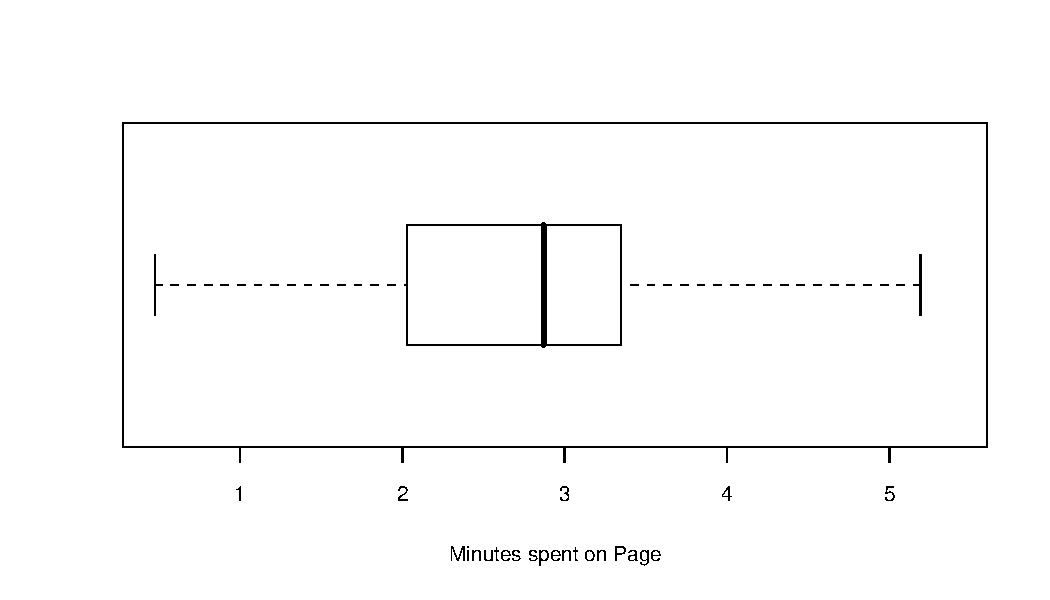
\includegraphics[width=0.5\textwidth]{timespentonpage}
}{
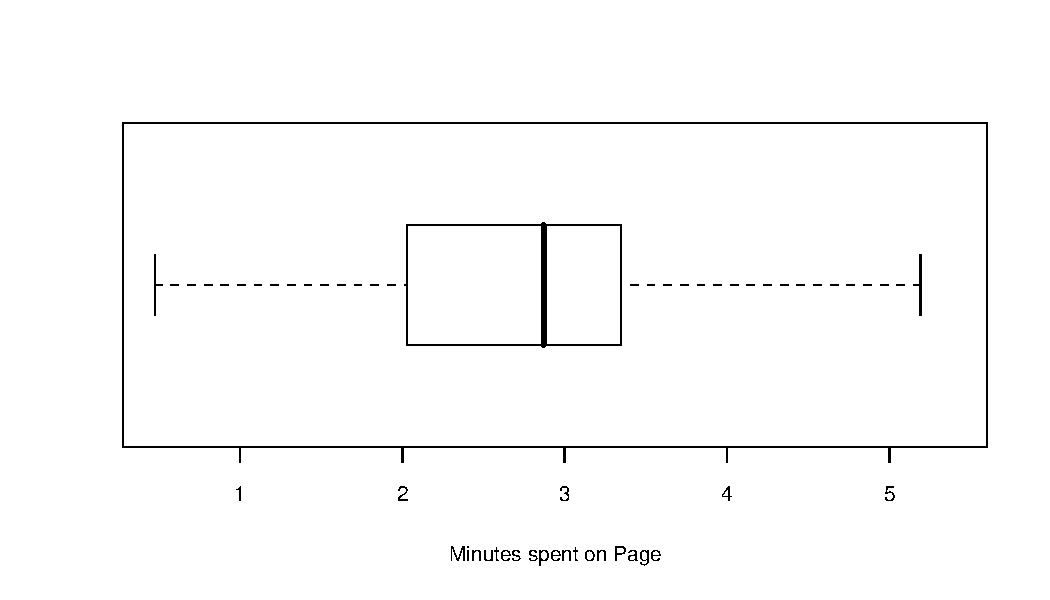
\includegraphics[width=0.8\textwidth]{timespentonpage}
}
\label{f:userstats}
\caption{Time spent for annotation of a single web page across all annotators of the \textit{Canola} corpus.}
\end{figure}

The data obtained from user annotations was next merged into a single corpus using the Applications \textit{merge} function (c.f. \ref{merge}), resulting of a total of 216 corpus pages, each backed by up to 8 user submissions.
Different treatment of JavaScript on the client side resulted in partial misalignment on some pages:
dynamic client code had inserted or re-ordered nodes in some instance while not in others.
We extended the merge procedure to accept some fuzziness in node matching, but still lost data from about 5\% of submissions that could not be re-aligned.
Until this problem is solved, we recommend to turn off JavaScript for web content via the Firefox Add-On.
Note that attaching unique IDs to text nodes is only a partial solution to this problem:
A common JavaScript idiom is to clone an existing element and to populate it with new content, ultimately leading to different nodes with the same ``unique'' ID. 

\begin{figure}[h]
\centering
\jss{
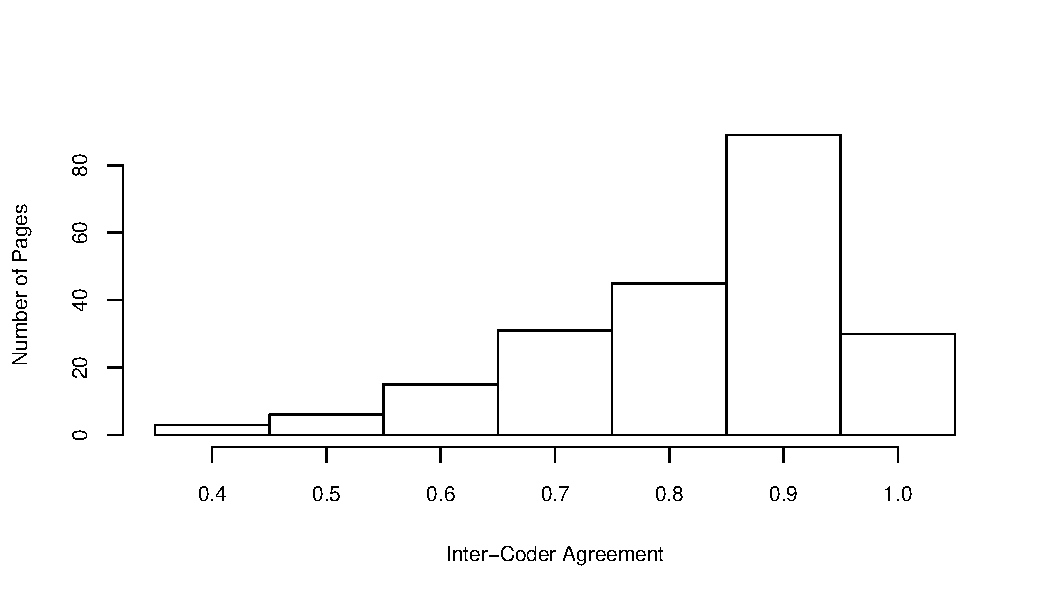
\includegraphics[width=0.5\textwidth]{agreementonpages}
}{
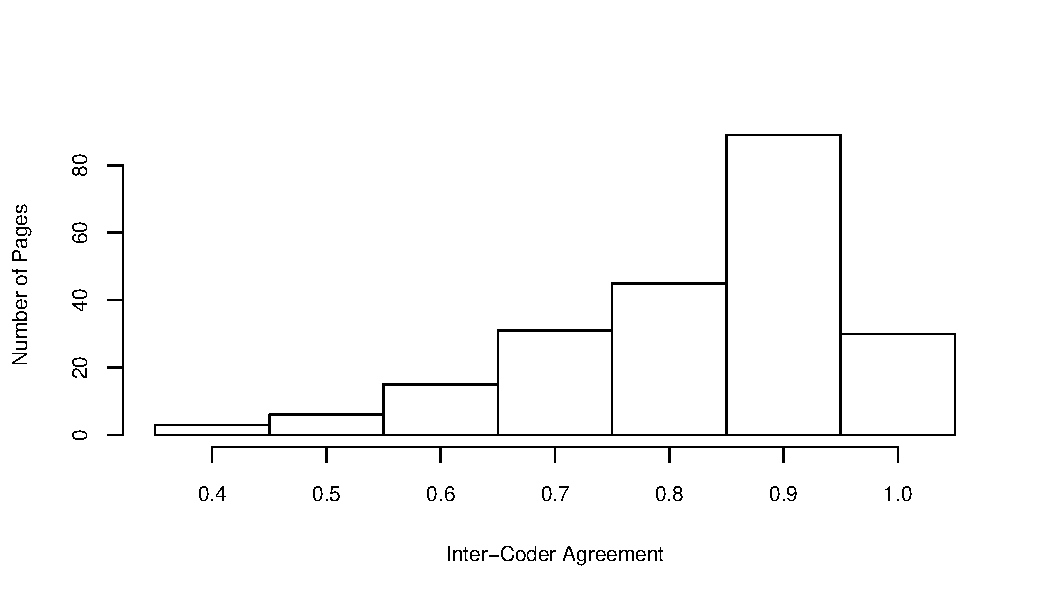
\includegraphics[width=0.8\textwidth]{agreementonpages}
}
\label{f:merge}
\caption{Agreement between submissions for one page over the \textit{Canola} corpus.}
\end{figure}


\subsection{Extraction Pipeline}

Feature Extraction commences by running the {\KrdWrd} application extraction pipeline over the merged data obtain from annotation. 
For the \textit{Canola} corpus' 216 pages, it took 2.5sec on average per page to generate text (2.5m characters total), DOM information (46575 nodes total), screen-shots (avg. size 997x4652px) and a file with the annotation target class for each text node.

We only used the stock {\KrdWrd} features on the DOM tree and visual pipeline, with a simple JAMF graph as a showcase (c.f. figure \ref{f:jamfgraph}).
For computing textual features, we stole Victors gut \cite{spoustamarekpecina2008}.

\begin{figure}[h]
\centering
\jss{
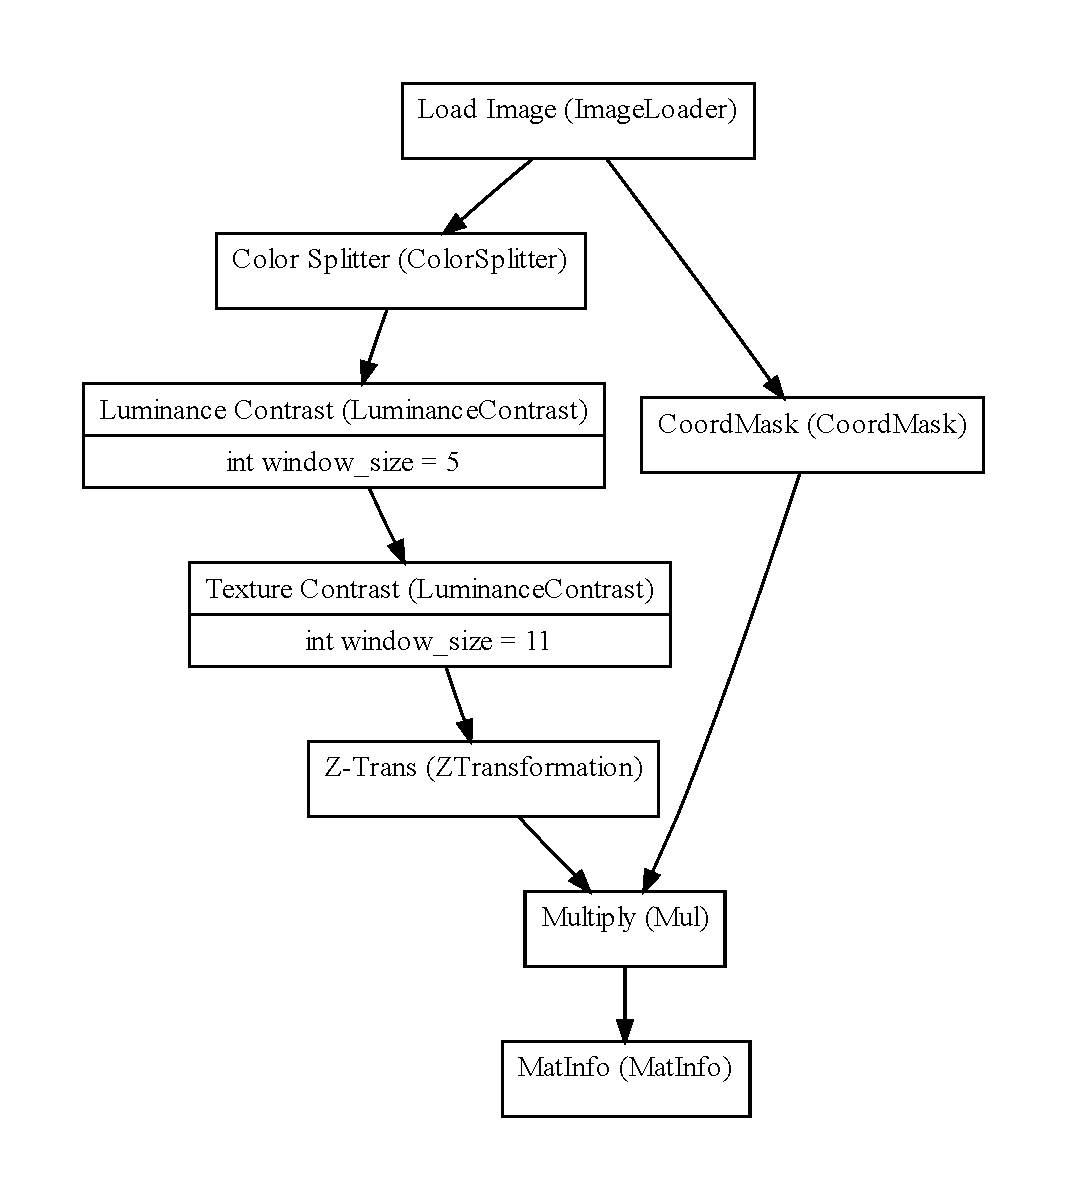
\includegraphics[width=0.4\textwidth]{jamfgraph}
}{
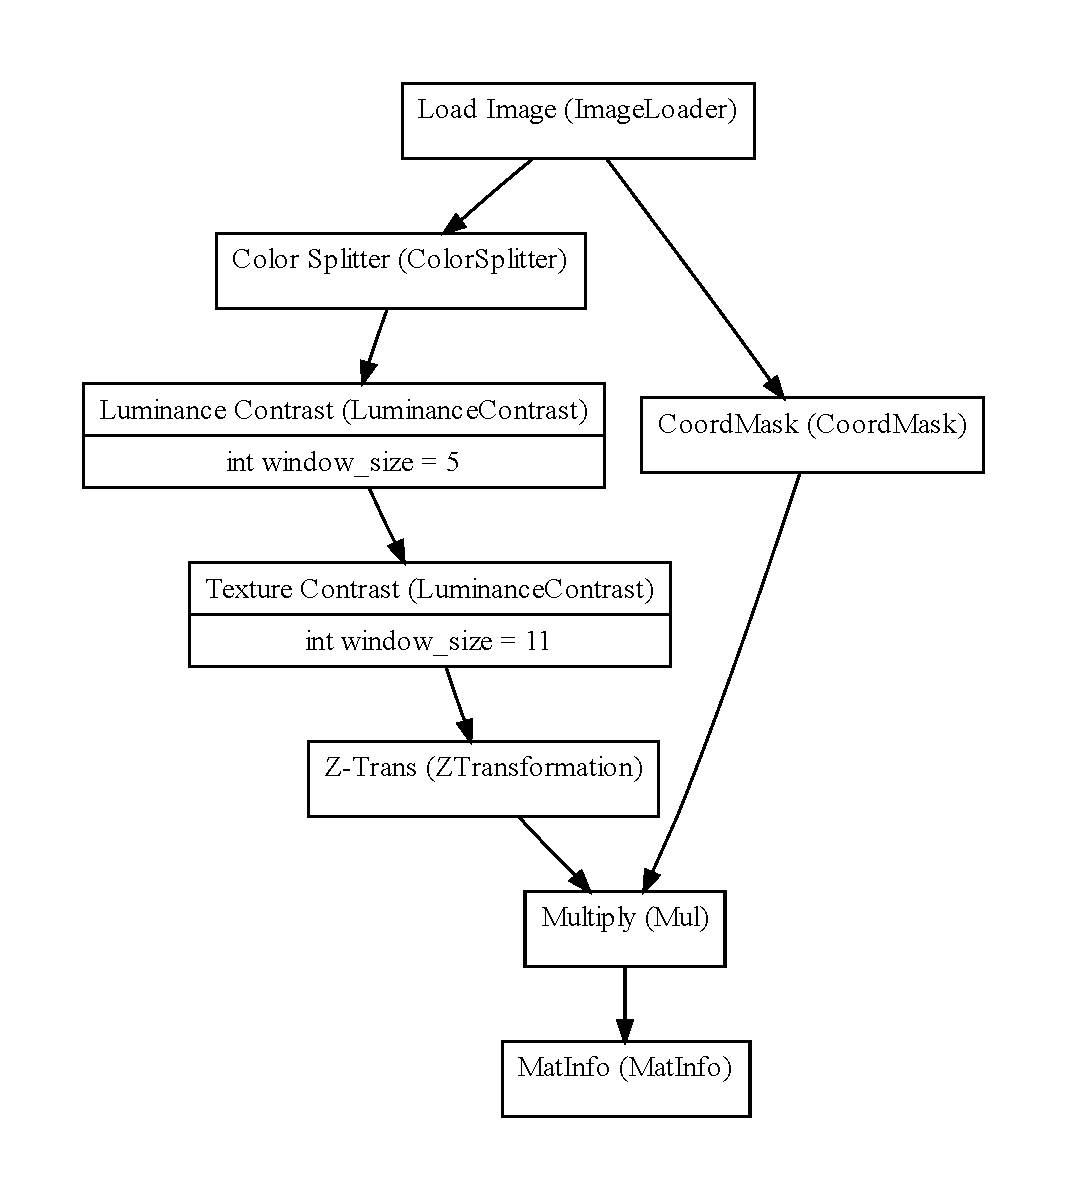
\includegraphics[width=0.6\textwidth]{jamfgraph}
}
\label{f:jamfgraph}
\caption{The simple JAMF graph used for the case study}
\end{figure}

\subsection{Experiment}

We used the data gathered by feature extraction for training a Support Vector Machine \cite{libsvm}.
We used an RBF kernel with optimal parameters determined by a simple grid search on a per-pipeline basis.
The total number of feature vectors corresponded to the number of text nodes in the corpus and was 46575.
Vector lengths for the different pipelines and test results from 10-fold cross validation are shown in table \ref{t:res}.

\begin{table}
\label{t:res}
\jss{
\caption{Classification Results for \textit{Canola} data set\\}}{
\captionabove{Classification Results for {\it Canola} data set}}
\jss{}{\sffamily\centering}
\begin{tabular}[h]{l|c|rrr}
Modules & \jss{Feat.}{Number of Features} & \jss{Acc.}{Accuracy} & \jss{Prec.}{Precision} & \jss{Recall}{Recall} \\
\hline
cl         & 21 & 84\% & 60\% & 70\% \\
dom        & 13 & 65\% & 64\% & 56\% \\
viz        &  8 & 86\% & 64\% & 82\% \\
cl dom     & 34 & 67\% & 74\% & 57\% \\
dom viz    & 21 & 67\% & 72\% & 59\% \\
cl viz     & 29 & 85\% & 60\% & 74\% \\
cl dom viz & 42 & 68\% & 76\% & 58\% \\
\end{tabular}
\end{table}

(new results yet to come in here, wait with interpretation...)

\subsection{Inspecting Classifier Results}

The classification results can be back-projected into the DOM-trees using the Application's \textit{diff} function.
As in the tutorial for annotators, it produces a visual diff, showing where the classifier failed.
Note that these results are just web pages, so they can be viewed anywhere without the help of the Add-on.
This quickly turned out to be a valuable tool in evaluation of classification results.

\section{\label{sec:limitations}Conclusions\label{conc}}

Employing {\KrdWrd} in the \textit{Canola} case study showed that we achieved what we set out for and gave some valuable experience for possible improvements:

The {\KrdWrd} Firefox Add-On is the first tool for web page annotation that integrates flawlessly into a users daily browsing experience.
It is unobstrusive and has a simple and intuitive user interface.
Users quickly learn how to annotate and produce quite uniform results, given sufficient annotation guidelines.

The {\KrdWrd} application and supporting infrastructure are a reliable platform under a real-world usage scenario.
By decoding any input data to UTF-8 at the moment it enters the system and ensuring that we explicitly deliver UTF-8 exclusively throughout the system, we circumvented all usual encoding problems.


The overall handling of JavaScript is not satisfactory.
To address the diversions between submits occurring after dynamic client-side JavaScript execution, the Add-on could hook into the node creation and clone processes.
They could be suppressed entirely or newly created nodes could grow a special id tag that help identifying them later.

For result analysis, we would like to expand the visual diff generated from classification results.
Showing results from separate runs on different subsets of the data or different parameters on one page would facilitate manual data inspection.
Presenting selected feature values per node might also help in developing new feature extractors, especially in the DOM context.


Summarizing, we have designed and implemented an architecture for holistic treatment of web pages in classification tasks.
We demonstrated that the KrdWrd system can be used to automatically build an annotated corpus from user submissions.
We also showed its broad set of extractable features, text, structure and imagery, and their contribution to classification.

\review{
%\section*{Acknowledgments}

}

